\documentclass[a4paper,12pt]{article}
\usepackage[a4paper,top=1.3cm,bottom=2cm,left=1.5cm,right=1.5cm,marginparwidth=0.75cm]{geometry}
%%% Работа с русским языком
\usepackage{cmap}					% поиск в PDF
\usepackage{mathtext} 				% русские буквы в фомулах
\usepackage[T2A]{fontenc}			% кодировка
\usepackage[utf8]{inputenc}			% кодировка исходного текста
\usepackage[english,russian]{babel}	% локализация и переносы

\usepackage{graphicx}
\usepackage{mathtools}
\usepackage{wrapfig}
\usepackage{tabularx}
\usepackage{amssymb}
\usepackage{hyperref}
\usepackage[rgb]{xcolor}
\hypersetup{colorlinks=true,urlcolor=blue}
\setcounter{secnumdepth}{0}
%% Шрифты
\usepackage{euscript}	 % Шрифт Евклид
\usepackage{amsmath}
\usepackage{mathtools}
%%% Заголовок
\author{Tsvetkova Amelia}
\title{Лабораторная работа по общей физике}

\date{\today}
\begin{document}
\begin{titlepage}
    \newpage
    \begin{center}
    {\large МОСКОВСКИЙ ФИЗИКО-ТЕХНИЧЕСКИЙ ИНСТИТУТ (НАЦИОНАЛЬНЫЙ ИССЛЕДОВАТЕЛЬСКИЙ УНИВЕРСИТЕТ)}
    \vspace{1cm}

    {\largeФизтех-школа аэрокосмических технологий}
    \vspace{6em}
    \end{center}
    
    \vspace{1.2em}

    \begin{center}
    \Large Лабораторная работа №5.1.2 \\
    Исследование эффекта Комптона
    \linebreak
    \end{center}
    
    \vspace{11em}
    
    \begin{flushright}
                       {\large Работу выполнила\\
                       Цветкова Амелия Антоновна\\
                       Б03-305 }
    \end{flushright}

    \vspace{\fill}

    \begin{center}
    Долгопрудный, 2025
    \end{center}

    \end{titlepage}

\section{Цели работы}
\begin{enumerate}
    \item Исследовать энергетический спектр $\gamma$-квантов, рассеянных на графите, с помощью сцинтилляционного спектрометра;
    \item Определить энегию рассеянных $\gamma$-квантов в зависимости от угла рассеяния;
    \item Определить энергию покоя частиц, на которых происходит комптоновское рассеяние.
\end{enumerate}

\section{Теоретические сведения}
В составе рассеянного излучения $\gamma$-лучей, измеренного Комптоном, кроме исходной волны с частотой $w_0$ появляется дополнительная длинноволновая компонента. Появление этой компоненты объяснимо, если считать, что $\gamma$-излучение представляет собой поток квантов (фотонов), имеющих энергию $\hbar w$ и импульс $p=\hbar w/c$.

\textbf{Эффект Комптона} - увеличение длины волны рассеянного излучения по сравнению с падающим - интерпретируется как результат упругого соударения двух частиц: $\gamma$-кванта и свободного электрона.

Рассмотрим элементарную теорию эффекта Комптона. Пусть электрон до соударения покоился (его энергия равна энергии покоя $mc^2$), а $\gamma$-квант имел начальную энергию $\hbar w_0$ и импульс $\hbar w_0/c$. После соударения электрон приобретает энергию $\gamma mc^2$ и импульс $\gamma mv$, где $\gamma = \frac{1}{\sqrt{1-v^2/c^2}}$, а $\gamma$-квант рассеивается на некоторый угол $\theta$ по отношению к первоначальному направлению движения. Энергия и импульс $\gamma$-кванта становятся соответственно равными $\hbar w_1$ и $\hbar w_1/c$.

Законы сохранения энергии и импульса:
$$
mc^2+\hbar w_0 = \gamma mc^2 + \hbar w_1,
$$
$$
\frac{\hbar w_0}{c} = \gamma mv\cos{\varphi} + \frac{\hbar w_1}{c}\cos{\theta},
$$
$$
\gamma mv\sin{\varphi} = \frac{\hbar w_1}{c}\sin{\theta}.
$$

Переходя от частот $w_0$ и $w_1$ к длинам волн $\lambda_0$ и $\lambda_1$:
\begin{equation}
    \Delta\lambda = \lambda_1-\lambda_0 = \frac{h}{mc}(1-\cos{\theta})=\Lambda_k(1-\cos{\theta}),
\end{equation}\label{1}

где $\lambda_0$ и $\lambda_1$ - длины волн $\gamma$-кванта до и после рассеяния, а величина
$$
\Lambda_k = \frac{h}{mc}=2,42\cdot 10^{-10}\text{см}
$$
называется \textbf{комптоновской длиной волны электрона}.

\begin{figure}[h]
\centering
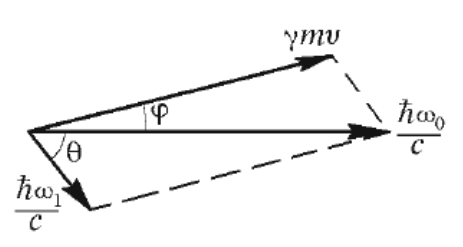
\includegraphics[width=0.4\linewidth]{img1.png}
\caption{Векторная диаграмма рассеяния $\gamma$-кванта на электроне}
\label{img1}
\end{figure}

Из формулы (1) следует, что комптоновское смещение не зависит ни от длины волны первичного излучения, ни от рода вещества, в котором наблюдается рассеяние.

При контоновском рассеянии каждый электрон атома ведет себя независимо от других, поскольку рассеяние в этом случае происходит на каком-либо одном из атомных электронов. При рэлеевском рассеянии фотоны излуччаются всеми электронами атомной оболочки, колеблющимися синфазно.

Основной целью данной работы является проверка соотношения (1). Преобразуем формулу (1) от длин волн к энергии $\gamma$-квантов:
\begin{equation}
    \frac{1}{\varepsilon(\theta)}-\frac{1}{\varepsilon_0}=1-\cos{\theta}
\end{equation}

Здесь $\varepsilon_0=E_0/(mc^2)$ - выраженная в единицах $mc^2$ энергия $\gamma$-квантов, падающтх на рассеиватель, $\varepsilon(\theta)$ - выраженная в тех же единицах энергия квантов, испытавших копмтоновское рассеяние на угол $\theta$, $m$ - масса электрона.

\section{Экспериментальная установка}

Источником излучения 1 служит $^{137}\text{Cs}$, испускающий $\gamma$-лучи с энергией 662 кЭв. Он помещен в толстостенный свинцовый контейнер с коллиматором. Сформированный коллиматором узкий пучок $\gamma$-квантов попадает на графитовую мишень 2.

\begin{figure}[h]
\centering
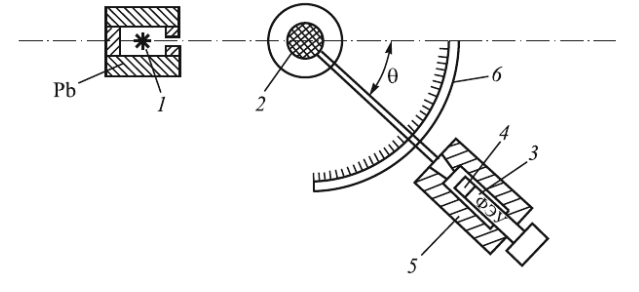
\includegraphics[width=0.4\linewidth]{img2.png}
\caption{Векторная диаграмма рассеяния $\gamma$-кванта на электроне}
\label{img2}
\end{figure}

Кванты, испытавшие комптоновское рассеяние в мишени, регистрируются сцинтилляционным счетчиком. Он состоит из фотоэлектронного умножителя 3 (ФЭУ) и сцинтиллятора 4. Сцинтиллятором служит кристалл NaI(Tl) цилиндрической формы диаметром 40 мм и высотой 40 мм, его выходное окно находится в оптическом контакте с фотокатодом ФЭУ. Сигналы, возникающие на аноде ФЭУ, подаются на ЭВМ для амплитудного анализа. Кристалл и ФЭУ расположены в светонепроницаемом блоке, укрепленном на горизонтальной штанге. Штанга вместе с этим блоком может вращаться относительно мишени, угол поворотаотсчитывается по лимбу 6.

Головная часть сцинтилляционного блока закрыта свинцовым коллиматором 5, который формирует входной пучок и защищает детектор от постороннего излучения.

При работе ФЭУ в спектрометрическом режиме величина выходного электрического импульса, снимаемого с анода ФЭУ, пропорциональна энергии регистрируемого $\gamma$-кванта. Световая вспышка в сцинтилляторе вызывается не самими $\gamma$-квантами, а образующимися в кристалле под действием $\gamma$-квантов электронами. Процесс преобразования энергии $\gamma$-кванта в определенное число фотонов на выходе сцинтиддятора состоит из трех стадий: рождение быстрых электронов, возбуждение атомов и молекул сцинтиллятора этими электронами и излучение световых фотонов возбужденными атомами и молекулами. Существуют три механизма взаимодействия $\gamma$-квантов с веществом: комптоновское рассеяние, фотоэффект и рождение электор-позитронных пар.

\section{Ход работы}
\begin{enumerate}
    \item Включаем все измерительные устройства и компьютер;
    \item Запускаем программу и входим в режим измерения спектра;
    \item Проверяем функционированпие установки в этом режиме при малом времени экспозиции (порядка 1 минуты) и снимаем спектр при $\theta=0^\circ$
    \item Проделываем измерения при $\theta$ с шагом $10^\circ$ до $110^\circ$
    \begin{table}[h!]
    \centering
    \begin{tabular}{||c||c|c|c|c|c|c|c|c|c|c|c|c|c|c||}
    \hline
    $\theta, ^\circ$ & 0 & 5 & 10 & 15 & 20 & 30 & 40 & 50 & 60 & 70 & 80 & 90 & 100 & 110 \\
    \hline
    $\sigma_\theta, ^\circ$ & 1 & 1 & 1 & 1 & 1 & 1 & 1 & 1 & 1 & 1 & 1 & 1 & 1 & 1 \\
    \hline
    $N$ & 875 & 916 & 847 & 901 & 760 & 644 & 578 & 506 & 451 & 395 & 351 & 310 & 294 & 270 \\
    \hline 
    $n$ & 6451 & 4863 & 3593 & 2615 & 1783 & 1914 & 1820 & 1672 & 1526 & 1387 & 1277 & 1184 & 1115 & 1043 \\
    \hline
    $\sigma_N$ & 0.29 & 0.34 & 0.39 & 0.46 & 0.55 & 0.54 & 0.55 & 0.57 & 0.60 & 0.63 & 0.65 & 0.68 & 0.70 & 0.73 \\
    \hline
    \end{tabular}
    \end{table}

    \item Оценим погрешность измерения номера канала следующим образом. Предположим, что форма пика близка к Гауссовой. Тогда: $\Delta \approx 2.35 \sigma_p$, где $\Delta$ - ширина пика на половине его высоты, $\sigma_p$ - стандартное отклонение, характеризующее ширину пика. Глядя на все пики на изображении, можно оценить, что их ширина на половине высоты составляет примерно 50-60 каналов. Возьмем для расчёта среднее значение: $\Delta\approx55$.

    Теперь рассчитаем стандартное отклонение пика: $\sigma_p \approx 23.4$ канала. 

    Погрешность определения математического ожидания (центра) гауссова распределения по $n$ измерениям равна: $\sigma_N = \sigma_p / \sqrt{n}$, где $n$ - интегральное количество отсчётов под пиком.

    Пример расчета погрешности для $\theta=0^\circ$: $\sigma_N = 23.4 /\sqrt{6451} \approx 0.29$ канала.
    

    \item Используя экспериментальные данные, построим график $\frac{1}{N(\theta)} -\frac{1}{N(0)}=A(1-\cos{\theta})$, откладывая по абсцисс величину $1-\cos{\theta}$, а по оси ординат величину $1/N(\theta)$ и ее ошибку. Проводим через полученные точки наилучшую прямую.
    \begin{table}[h!]
    \centering
    \begin{tabular}{||c|c|c|c|c|c|c|c||}
    \hline
    $\theta, ^\circ$ & $x=1-\cos{\theta}$ & $\sigma_x$ & $y = 1/N(\theta)$ & $\sigma_y$ \\ 
    \hline
    \hline
    0    & 0.0000 & 0.0000 & 1142.9 & 0.38  \\
    \hline
    5    & 0.0038 & 0.0015 & 1091.7 & 0.40  \\
    \hline
    10   & 0.0152 & 0.0030 & 1180.6 & 0.54  \\
    \hline
    15   & 0.0341 & 0.0045 & 1109.9 & 0.56  \\
    \hline
    20   & 0.0603 & 0.0060 & 1315.8 & 0.96  \\
    \hline
    30   & 0.1340 & 0.0087 & 1552.8 & 1.30  \\
    \hline
    40   & 0.2340 & 0.0112 & 1730.1 & 1.64  \\
    \hline
    50   & 0.3572 & 0.0134 & 1976.3 & 2.24  \\
    \hline
    60   & 0.5000 & 0.0151 & 2217.3 & 2.95  \\
    \hline
    70   & 0.6580 & 0.0164 & 2531.6 & 4.04  \\
    \hline
    80   & 0.8264 & 0.0172 & 2849.0 & 5.30  \\
    \hline
    90   & 1.0000 & 0.0175 & 3225.8 & 7.09  \\
    \hline
    100  & 1.1736 & 0.0172 & 3401.4 & 8.14  \\
    \hline
    110  & 1.3420 & 0.0164 & 3703.7 & 9.98  \\
    \hline
    \end{tabular}
    \end{table}

    \item С помощью графика с формулы: $mc^2=E(0)\frac{E(90)}{E(0)-E(90)}=E_\gamma\frac{N(90)}{N(0)-N(90)}$ определим энергию покоя частицы, на которой происходит комптоновское рассеяние первичных $\gamma$-квантов
    $$
    N(0) = 1/b \quad\quad\quad\quad\quad N(90)=1/(k+b)
    $$
    где $k$, $b$ - коэффициенты аппроксимирующей прямой 
    
    \begin{figure}[h]
    \centering
    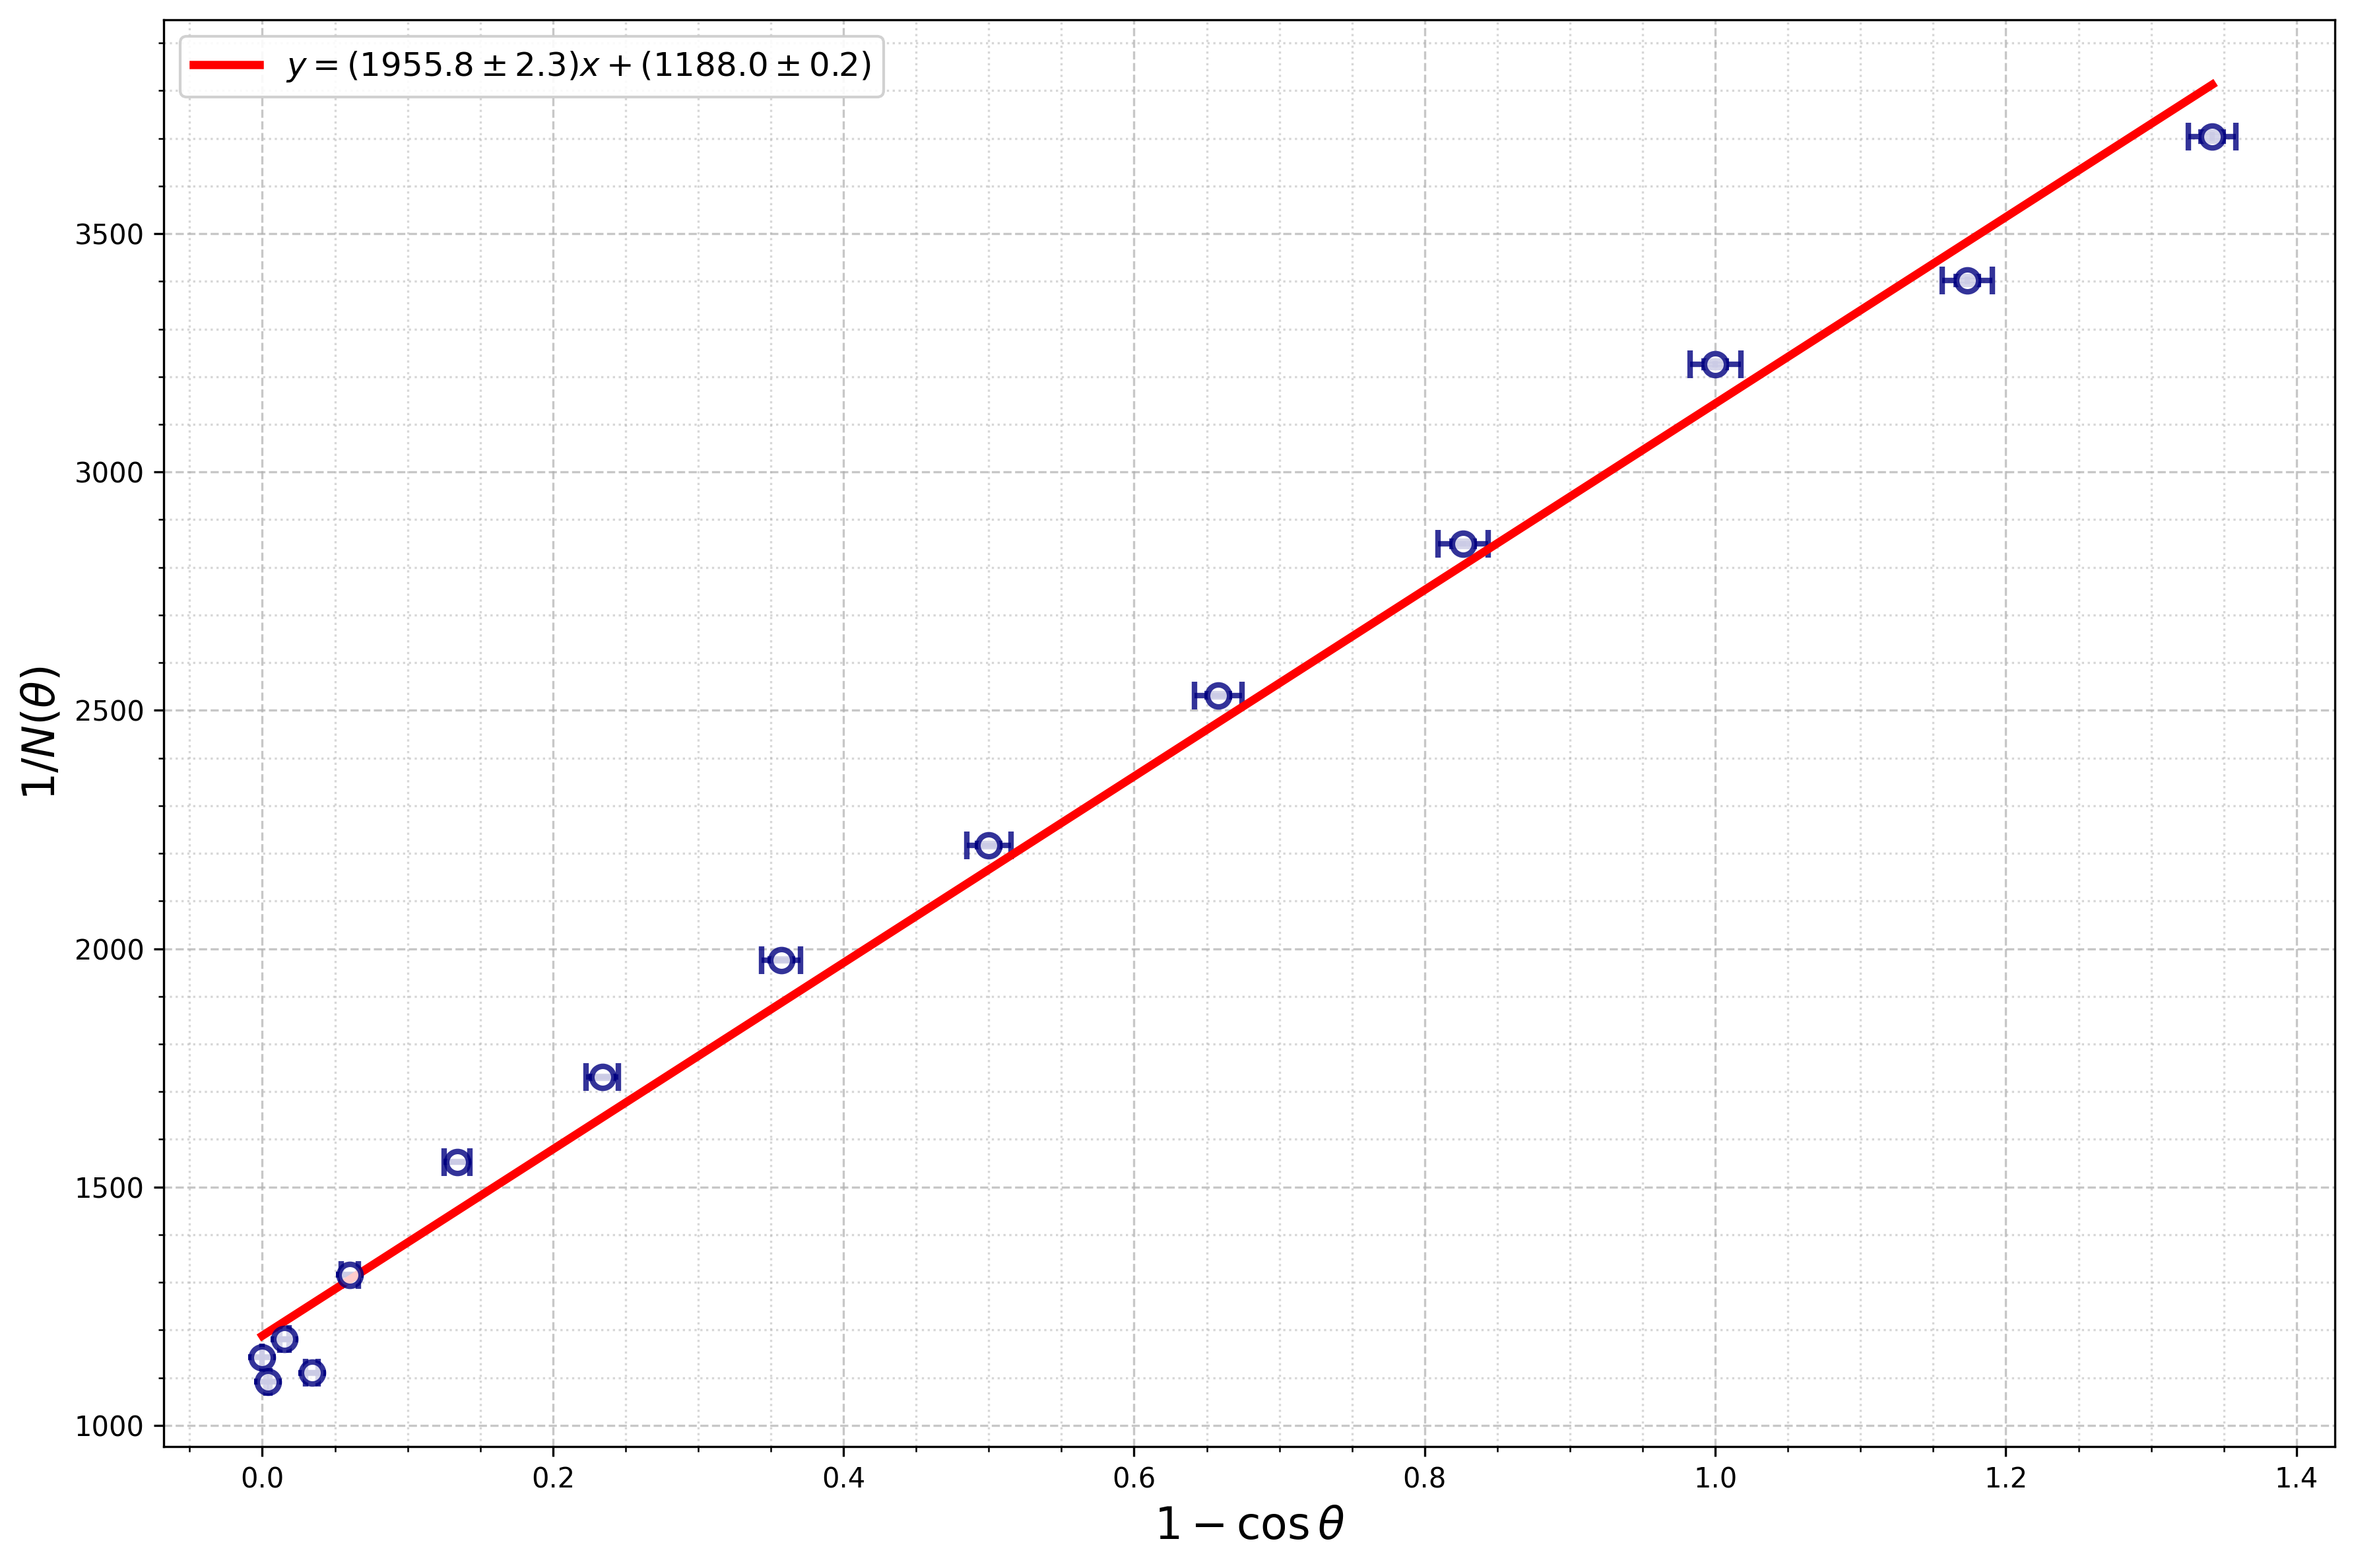
\includegraphics[width=1\linewidth]{1.png}
    \caption{Зависимость $1/N(\theta)$ от $(1-\cos{\theta})$}
    \label{graph1}
    \end{figure}
    
    Считаем $E_\gamma=662$кЭв
    
    $$
    mc^2 = E_\gamma \cdot \frac{N(90)}{(N(0) - N(90))}=402.13 \texttt{кЭв}
    $$
    $$
    \sigma_{mc^2}^2 = \left(\frac{\partial mc^2}{\partial E_\gamma}\right)^2 \sigma_{E_\gamma}^2 + \left(\frac{\partial mc^2}{\partial k}\right)^2 \sigma_k^2 + \left(\frac{\partial mc^2}{\partial b}\right)^2 \sigma_b^2
    $$
    где частные производные равны:
    
    $$
    \frac{\partial mc^2}{\partial E_\gamma} = \frac{N_{90}}{N_0 - N_{90}}
    $$
    $$
    \frac{\partial mc^2}{\partial k} = \frac{E_\gamma}{(k + b)^2} \cdot \frac{N_0}{(N_0 - N_{90})^2} 
    $$
    $$
    \frac{\partial mc^2}{\partial b} = \frac{E_\gamma}{(k + b)^2} \cdot \frac{N_{90}}{(N_0 - N_{90})^2}
    $$
    
    Подставляя производные, получаем итоговую формулу:
    
    $$
    \sigma_{mc^2}^2 = \left(\frac{N_{90}}{N_0 - N_{90}}\right)^2 \sigma_{E_\gamma}^2 + \left(\frac{E_\gamma}{(k + b)^2} \cdot \frac{N_0}{(N_0 - N_{90})^2}\right)^2 \sigma_k^2 + \left(\frac{E_\gamma}{(k + b)^2} \cdot \frac{N_{90}}{(N_0 - N_{90})^2}\right)^2 \sigma_b^2=3.05\texttt{кЭв}
    $$

    Табличное значение: $mc^2_\text{табличное}=511$кЭв. Отклонение: $21.31\%$

    \begin{center}
        \boxed{mc^2=(402.13\pm3.05)\text{кЭв}(\varepsilon=0.76\%)}
    \end{center}

\end{enumerate}

\section{Выводы}

В ходе работы был исследован энергетический спектр $\gamma$-квантов, рассеянных на графите с помощью сцинтилляционного спектрометра. Была доказана справедливость эффекта Комптона
в силу линейности графика.

Также была определена энергия покоя частиц, на которых происходит комптоновское рассеяния. Результаты совпадают по порядку величины, но в пределах погрешностей не совпадают. Это может быть вызвано недостаточной длительностью экспозиций при проведении эксперимента.

\section{Приложение}

\begin{figure}[h]
\centering
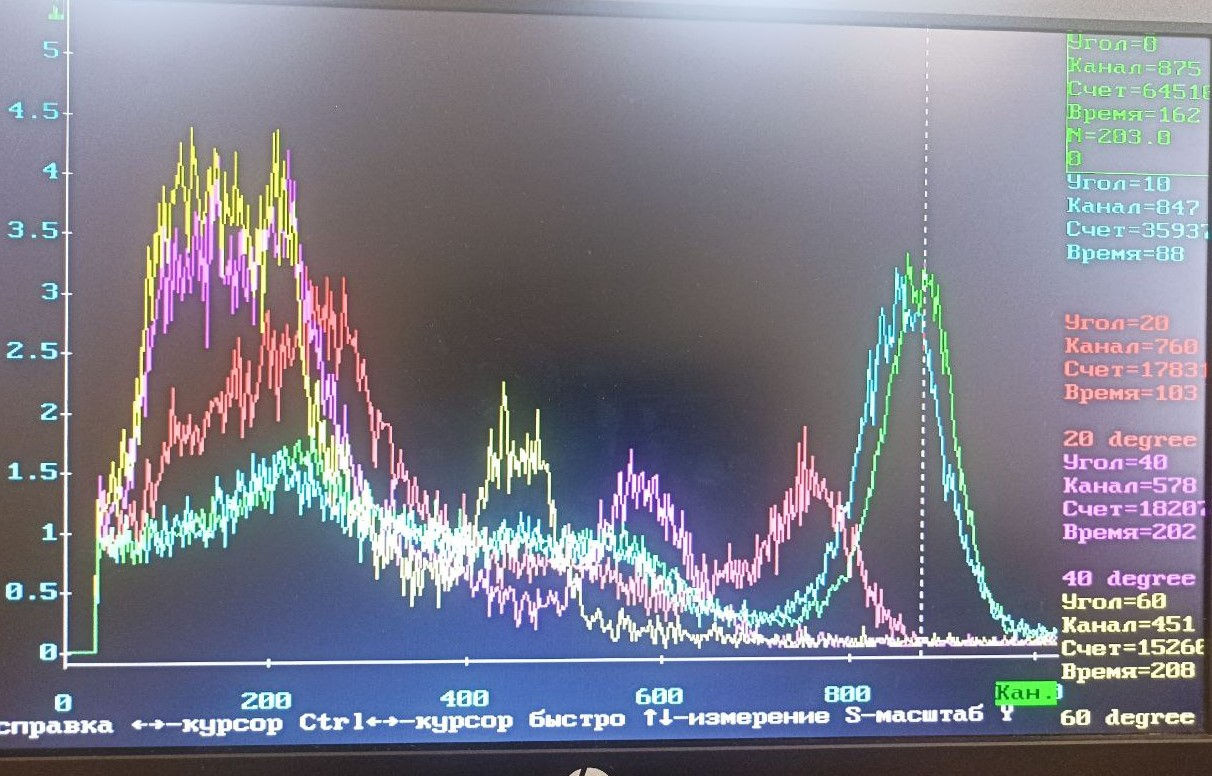
\includegraphics[width=1\linewidth]{comp.jpg}
\caption{Спектр при разных значениях угла $\theta$}
\label{comp}
\end{figure}

\end{document}
